\section{Sumador con acarreo de entrada \label{sec:s1}}

\begin{center}
	\begin{minipage}{12cm}
		\begin{tcolorbox}[title=Actividad 1]
			Completar el código de la lámina 10 para implementar el sumador con acarreo de entrada ($Ci$) y compilar. Usar el visor RTL para verificar cómo se implementa dicho sumador. ¿Cuántos sumadores se utilizan? Utilizar los dos lenguajes.
		\end{tcolorbox}	
	\end{minipage}
\end{center}

La visualización RTL del sumador con acarreo de entrada en VHDL se muestra en la \autoref{fig:adder_cin_vhdl_rtl} y en Verilog en la \autoref{fig:adder_cin_verilog_rtl}. Como se observa, si se realiza una descripción por comportamiento, el entorno utiliza dos instancias de sumadores de 2 entradas, ya que en el primero realiza la suma de A y B (ambos de 8 bits), mientras que el segundo sumador realiza la operación entre el resultado anterior y el acarreo de entrada (nótese que al ser el acarreo de entrada de un solo bit, pone los otros 7 bits restantes en cero con GND). Las simulaciones para el código en VHDL se visualizan en la \autoref{fig:adder_cin_vhdl_WaveBi} en base binaria y en la \autoref{fig:adder_cin_vhdl_WaveDe} en base decimal. En cambio, las simulaciones para el código en Verilog se visualizan en la \autoref{fig:adder_cin_verilog_WaveBi} en base binaria y en la \autoref{fig:adder_cin_verilog_WaveDe} en base decimal. Cabe resaltar que los valores utilizados para los bancos de pruebas fueron obtenidos de un generador de números aleatorios entre 0 y 255 \cite{numeros_2024}.

\begin{figure}[ht]
	\centering
	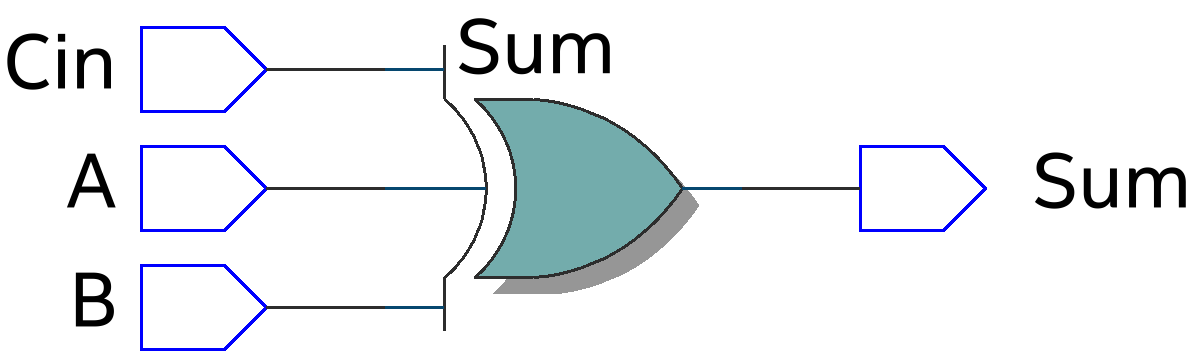
\includegraphics[scale=0.5]{Adder_Cin_VHDL_RTL.png}
	\caption{Diagrama RTL del sumador con acarreo de entrada en VHDL. \label{fig:adder_cin_vhdl_rtl}}
\end{figure}

\begin{figure}[ht]
	\centering
	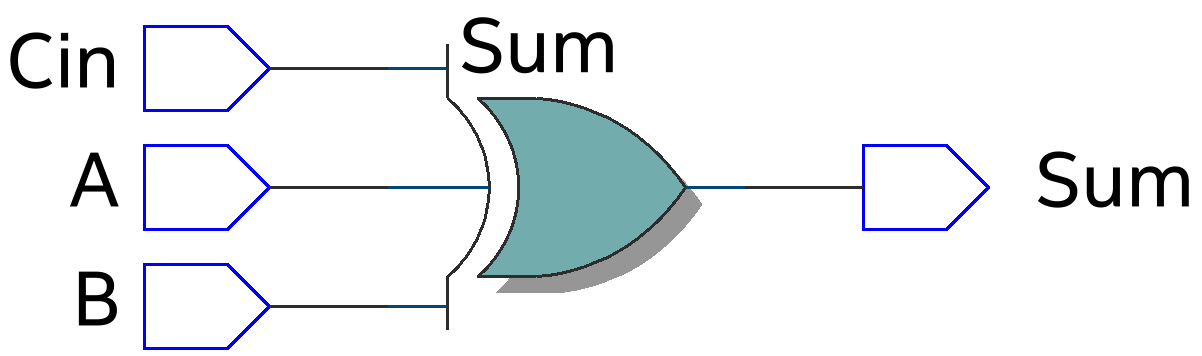
\includegraphics[scale=0.5]{Adder_Cin_Verilog_RTL.png}
	\caption{Diagrama RTL del sumador con acarreo de entrada en Verilog. \label{fig:adder_cin_verilog_rtl}}
\end{figure}

\begin{figure}[ht]
	\centering
	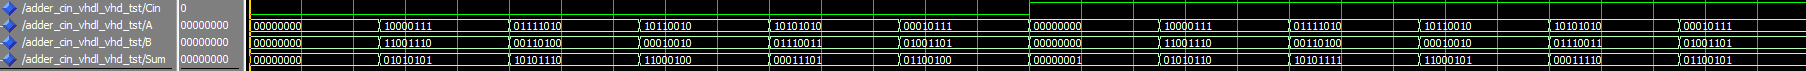
\includegraphics[scale=0.35]{Adder_Cin_VHDL_WaveBi.png}
	\caption{Simulación del sumador con acarreo de entrada en VHDL con el visor de formas de onda de ModelSim (Base binaria). \label{fig:adder_cin_vhdl_WaveBi}}
\end{figure}

\begin{figure}[ht]
	\centering
	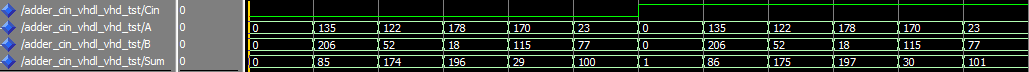
\includegraphics[scale=0.6]{Adder_Cin_VHDL_WaveDe.png}
	\caption{Simulación del sumador con acarreo de entrada en VHDL con el visor de formas de onda de ModelSim (Base decimal). \label{fig:adder_cin_vhdl_WaveDe}}
\end{figure}

\begin{figure}[ht]
	\centering
	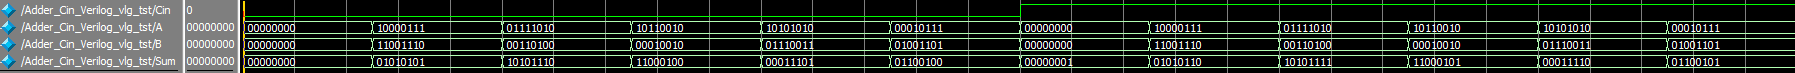
\includegraphics[scale=0.35]{Adder_Cin_Verilog_WaveBi.png}
	\caption{Simulación del sumador con acarreo de entrada en Verilog con el visor de formas de onda de ModelSim (Base binaria). \label{fig:adder_cin_verilog_WaveBi}}
\end{figure}

\begin{figure}[ht]
	\centering
	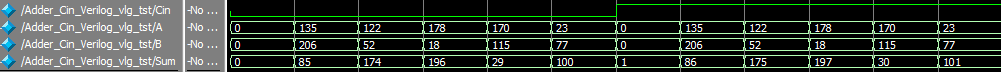
\includegraphics[scale=0.6]{Adder_Cin_Verilog_WaveDe.png}
	\caption{Simulación del sumador con acarreo de entrada en Verilog con el visor de formas de onda de ModelSim (Base decimal). \label{fig:adder_cin_verilog_WaveDe}}
\end{figure}
